\documentclass[BCOR=1mm, DIV=calc,10pt,
twoside=true,
twocolumn,
headings=normal]{scrartcl}
%\KOMAoptions{DIV=calc}% recalculate the page layout with a calculated DIV value

% Recommended, but optional, packages for figures and better typesetting:
\usepackage{microtype}
\usepackage{graphicx}
%\usepackage{subfigure}
\usepackage{booktabs} % for professional tables

\usepackage{amsmath}
\usepackage{bm}
\usepackage{url}

% Attempt to make hyperref and algorithmic work together better:
\newcommand{\theHalgorithm}{\arabic{algorithm}}

\usepackage{cite}
\usepackage{amsmath,amssymb,amsfonts}
%\usepackage{algorithmic}
\usepackage{graphicx}
\usepackage{textcomp}
\usepackage{xcolor}

\usepackage{authblk}


\newcommand{\fig}{Fig. }
\newcommand{\eqn}{Eqn. }
\newcommand{\tab}{Tab. }
\newcommand{\wrt}{w.r.t. }
\newcommand{\etal}{ {\em et al. }}


\begin{document}


\title{Demand Forecasting of individual Probability Density Functions with Machine Learning}

\author[1]{Felix Wick \thanks{felix.wick@blueyonder.com}}
\author[2]{Ulrich Kerzel \thanks{u.kerzel@iubh-fernstudium.de}}
\author[1]{Trapti Singhal \thanks{trapti.singhal@blueyonder.com}}
\author[1]{Martin Hahn \thanks{martin.hahn@blueyonder.com}}
\affil[1]{\small Blue Yonder GmbH (Karlsruhe, Germany)}
\affil[2]{\small IUBH Internationale Hochschule (Erfurt, Germany)}


\date{}

\maketitle

\begin{abstract}
Demand forecasting is a central component for many aspects of supply chain operations, as it provides crucial input for subsequent decision making like ordering processes. While machine learning methods can significantly improve prediction accuracy over traditional time series forecasting, the calculated predictions are often mere point estimations for the conditional mean of the underlying random distribution, and the most powerful approaches, like deep learning, are usually opaque in terms of how its individual predictions can be interpreted. We present an extension to our earlier work on a supervised machine learning method called Cyclic Boosting to predict full individual probability density functions in form of negative binomial distributions, that are fully explainable on the individual prediction level. Also, we describe new techniques for both qualitative and quantitative evaluation of predicted probability density functions by comparison with observed data.
\end{abstract}

{Keywords: \textbf{machine learning, demand forecasting}}

PDF
\section{Introduction}

Demand forecasting is one of the main challenges for retailers and at the core of business operations. Due to its stochastic nature, demand is difficult to forecast as it depends on many influencing factors and the realized demand can be interpreted as a random variable that is described by an appropriate probability density function (PDF). In order to make operational decisions, an optimal point estimator has to be defined, that can be used to derive ordering decisions used in the replenishment process of the retailer. Demand estimation is further complicated by the fact that retailers typically only observe realized sales rather than the actual demand, and in case the demand exceeds the current stock level the data become censored. The ordering decision process is complicated by a range of factors: Even in the case of accurate  demand forecasts, the decision maker has to balance conflicting metrics to reach an optimal decision: Ordering to few items may result in stockout situations leading to unrealized demand and unsatisfied customers. Ordering too many items results in excess inventory which increases transport and storage costs and, in the case of perishable goods, excessive waste, as spoilt items need to be disposed of at additional cost and potentially even environmental impact. This situation is particularly noticeable in the so called "ultra-fresh'' category, which includes items such as bakery products, ready-meals, fresh diary products, or certain meat products such as ground meat. These items typically have a shelf-life of less than a business day to a few business days at most, with a continuous spectrum depending on the exact item. In many situations, additional constraints have to be considered to reach an optimal ordering decision: Delivery cycles of items may vary depending on the type of item and the wholesaler or manufacturer from which they are procured. Retailers also operate at a given service level to guarantee that a certain level of demand can be fulfilled. The exact service level typically depends on the overall business policy of the retailer and may also depend on individual products, ranging from "never-out-of-stock'' items to a service level exceeding e.g. 90\%.

The availability of Big Data allows capturing, storing and processing a vast amount of data associated with demand, such as historic sales records, information about promotional events or advertisements, pricing information, local weather at retail locations, seasonal information as well as a wide range of further variables. Modern machine learning algorithms can then be used to predict the per-item demand distribution, corrected for censored data, from which an optimal point estimator can be derived to be used in the subsequent ordering decision. It is important to note that demand as a random variable is not identically and independently distributed (i.i.d.). While the probability distribution describing the demand can be attributed to a given family or parametrization, the exact parameters vary: Seasonal effects, finite life cycles of products and the introduction of new products influence the demand distribution, as well as the local weather at the retail location or the retail location itself in terms of size, assortment range, customer diversity and other factors. The retailers themselves also actively influence demand by using advertisements to highlight products, offering rebates or discounts for specific products as well as pursuing an active pricing strategy. This means that while we can generally assume that demand follows a specific type of probability distribution, its parameters are unique to the  instance for which an estimate is required. For example, the probability distribution governing the demand of a particular item is specific to the item, date and retail location for which the forecast is made and depends on a wide range of further influencing factors.

The remainder of the paper is organized as follows: We first review the relevant literature and existing work in sec. \ref{sec:LitRev}. We then describe our method to predict individual negative binomial PDFs by means of a parametric approach including two distinct machine learning models for mean of variance in sec. \ref{sec:pdfEstimation}. After that we describe methods for the qualitative and quantitative evaluation of PDF predictions in sec. \ref{sec:pdfEvaluation}. And finally, we present a demand forecasting example to show an application of our methods in sec. \ref{sec:example}.


\section{Literature Review}
\label{sec:LitRev}

Inventory management offers a rich theory and the extensive body of research can be broadly grouped into two categories, where the inventory control problem is either based on some knowledge of the underlying demand  distribution or an integrated approach that seeks to map directly from the available data (historic sales records and further variables) to the ordering decision. This approach is often referred to as "data-driven newsvendor'' and discussed  e.g. in \cite{beutel2012safety,ban2019big,bertsimas2020predictive, oroojlooyjadid2020applying}. It aims to avoid estimating the underlying probability distribution and use the available data to derive the operational decisions directly.  An overview of a range approaches can also be found in \cite{huber2019data}.

Although this approach seems preferable at first glance, since it avoids determining the full demand distribution and results directly in the desired operational decision (the order quantity), it faces several drawbacks. First of all, the full probability distribution for the demand of a specific item at a given sales location and business day includes all available information including the uncertainty of the modelled demand. This can be used to simulate the performance on a per-item level and e.g. optimize the impact on business strategy decisions on conflicting metrics such as stock out- and waste-rate. By forecasting the full demand distribution as opposed to point estimators such as the expected demand or the median of the distribution, the forecast quality can be evaluated for quantiles of the distribution, including the often extensive tails of the distribution. Additionally, a purely data-driven approach going from the observed data directly to the operational decision (such as the order quantity) does not allow to analyze the data-generating process, i.e. the mechanism behind the stochastic behavior of the customer demand. However, modelling demand directly is vital if a causal analysis is planned at a later stage or independently, for example to study the effect promotions, advertisements,  price changes or other influencing factors in either Pearl's do-calculus \cite{PearlCausality} or Rubin's potential outcomes framework \cite{rubin1974estimating}. Using an operational quantity such as the order quantity will in most cases be an insufficient proxy of the quantity of interest (customer demand) and likely lead to unnecessary causal pathways that may not be able to be fully controlled for. From a practical perspective, separating the demand forecast from the operational decisions (i.e. calculating the  order quantities for the next delivery cycle) also allows to evaluate longer-term planning and reduces the complexity as it avoids coupling the complex delivery schedules of multiple wholesalers and manufacturers with the forecast of customer demand. This also allows to share long-term demand predictions with other business units or external vendors  and wholesalers to ease their planning for the production and supply-chain processes upstream of the retailer. From the perspective of industrial practice, modelling the demand separately from deriving the subsequent orders  has the additional benefit that multiple retail chains can benefit from any improvement in the model description even if the concrete retailers are unrelated to each other. For example, if a particular effect was identified at some retailer A and included in the machine learning model, the improvement can be rolled out immediately or on request to all other retailers using this system on a planetary scale without having to adapt the underlying machine learning model for each retailer individually.

In contrast to the direct mapping the observed data to ordering decisions, more traditional inventory control systems rely on the knowledge of the demand distribution in one form or another, see e.g. \cite{silver1998} for an overview. In $(s,S)$ type inventory control systems \cite{Scarf1958}, inventory levels are monitored at regular intervals and orders are dispatched once the inventory level reaches a minimal value $s$. In case of linear holding and shortage costs, such policies are optimal \cite{Scarf1959}, although perishable goods pose more challenges, see e.g. \cite{Nahmias1973,Nahmias1975,nahmias1978}. Additionally, service level constraints can be included in these kind of inventory control systems \cite{minner2010periodic}. Perishable goods are well described by the "newsvendor-problem'' \cite{Edgeworth}, where in the simplest case all stock perishes at the end of the selling period (e.g. a business day). For a detailed review of the newsvendor problem see e.g. \cite{Khouja1999537}. Assuming linear underage and overage costs $b,h >0$, the optimal quantile $q_{\mathrm{opt}} = {b}/{(b+h})$ of a known demand distribution $f(D)$ can be calculated exactly.

The main objective in any of these approaches is to determine the underlying demand distribution. The simplest approach is to just use the observed sales events and forecast these as a time series (see e.g. \cite{alwan2016}) or via sample average approximation (SAA), see e.g. \cite{shapiro2014} for an overview. However, these approaches do not make use of any data apart from the sales record themselves, although we know that many variables such as price or advertisements influence, and therefore are highly correlated with, the demand. Saghafian and Tomlin \cite{saghafian2016newsvendor} propose to include partial information about the distribution in the derivation of the operational decision, i.e. the  calculation of the optimal order quantity.

However, in order to be able to fully optimize the operational decision, it is critical that one indeed reconstructs a full demand distribution. This also implies that a simple point-estimator, as provided by the most common statistical techniques and machine-learning approaches, will not suffice. Additionally, we need to consider that demand is not i.i.d., but depends on external factors such as season, weather, product life-cycle, and is also actively changed by the retailer by setting a specific price, offering rebates or running advertisements. Additionally, the demand implicitly depends on the location of the retail outlet as well as the specifics of that location, such as product  assortment influencing the choice of possible replacement articles and many more. These complications are the main reason we cannot treat the replenishment process as $n$ independent newsvendor-type problems.

Instead, we need to determine the full demand distribution from data, conditional on the relevant variables such as date, location, and item, taking all auxiliary data such as article characteristics, pricing, advertisements, retail location details, etc. into account. This can be done in several ways: Quantile regression \cite{koenker2001, wen2017} can be implemented in various frameworks and used to estimate a range of quantiles for each predicted distribution from which an empirical probability distribution can be interpolated. Using a dedicated neural network \cite{Feindt2006190}, either the  full probability distribution or a defined range of quantiles can be calculated directly from the data for each individual prediction without assuming an underlying model. Alternatively, one can assume a given demand model and fit the model parameters instead of reconstructing the complete distribution \cite{astonpr373, SALINAS20201181}. This approach is computationally favourable, as fewer parameters need to be estimated compared to the case of the full distribution. Empirically, one can determine the best fitting distribution from data \cite{adan1995}. However, given the stochastic nature of the demand, such an empirically determined distribution is not expected to be stable and prone to sudden changes. Instead, the choice of the demand distribution should be motivated by theoretic considerations. The discrete demand is typically modelled as a negative binomial distribution (NBD), also known as Gamma-Poisson distribution \cite{Ehrenberg1959,Ehrenberg1967,Ehrenberg1972,Chatfield1973,Schmittlein_1985}. This distribution arises if the Poisson parameter $\mu$ is a random variable itself that follows a Gamma distribution. The NBD has two parameters, $\mu$ and $ \sigma^2 > \mu$, and is over-dispersed compared to the Poisson distribution for which $\mu = \sigma^2$. Hence, for each ordering decision, the model parameters $\mu$ and $\sigma$ need to be determined for each item at the required granularity, typically for each sales location and ordering time, depending on all auxiliary data describing article details, retail location, and influencing factors such as pricing and advertisement information.

\subsection*{Summary of Contributions}

In the following, we will demonstrate how the explainable machine learning algorithm Cyclic Boosting \cite{Wick2019} can be used to model the demand distribution at the granularity needed by the retailer. Typically this means that the full demand distribution has to be estimated per SKU for each sales location and opening day, conditional on a wide range of variables such as weather, prices, promotions, etc. In contrast to using a "black-box'' machine learning model, using Cyclic Boosting allows to interpret how each individual prediction was made and what the most important variables are per individual prediction.

Additionally, we show how the cumulative distribution function (CDF) or inverse quantiles can be used to accurately asses the forecast quality of the full predicted demand distribution, including the tails of the distribution. This allows to verify that the predicted demand distribution accurately reflects the observed data and can hence be used both to derive operational decisions such as  order quantities as well as strategic business decisions by the retailer.


\section{Negative Binomial PDF Estimation}
\label{sec:pdfEstimation}

To predict an individual PDF by means of a parametric approach, one has to rely on a model assumption about the underlying distribution of the random variable to be predicted. In the following, we describe such a parametric approach with the model assumption of a negative binomial probability distribution. For a PDF prediction under a negative binomial model assumption, there is the need for the estimation of two parameters, for example its mean and its variance.

This can be done using two independent models, one to estimate the mean and the other for the variance. At least in principle, any method can be used. However, as argued above, in the case of demand forecasting, each prediction is highly specific to the circumstances in which it is used (such as product ID, date, and store location) and may depend on  a multitude of describing variables (features). Machine learning algorithms are ideally suited for this task and in the following we will use the Cyclic Boosting algorithm.

This means we use two subsequent, independent Cyclic Boosting models in order to estimate individual PDFs, the first to estimate the mean and the second to estimate the variance. The features may or may not differ between the mean and variance estimation models. But in any case, as there is a strong correlation between mean and variance, it is beneficial to include the corresponding predicted mean from the mean model as feature in the variance model. The assigned mean and variance predictions can then be used to generate individual PDFs according to a functional negative binomial distribution assumption for each sample. While any machine learning algorithm outputting a conditional mean as prediction may be used to get an approximate estimate for the mean of an underlying negative binomial distribution, it is preferable to choose an algorithm using a negative binomial assumption for its inner regularization methods, like Cyclic Boosting in multiplicative regression mode.

In the following, after a brief recap of the fundamental ideas of Cyclic Boosting, we describe a method to predict the variance of a negative binomial PDF along with its mean individually for each sample by means of Cyclic Boosting.

\subsection{Cyclic Boosting Recap}
\label{sec:CB}

In our earlier work \cite{Wick2019}, we have presented a new machine learning algorithm, Cyclic Boosting, which can be categorized as a generalized additive model with a cyclic coordinate descent optimization featuring a boosting-like update of parameters. The major benefits of Cyclic Boosting are that it is not only extremely performant in practical applications, like demand forecasting, at large scale, but also fully explainable. Traditional machine learning algorithms are typically "black box'' approaches, where the individual decision cannot be explained. Cyclic Boosting on the other hand allows to follow how each individual prediction was made. The main idea of this algorithm is the following: When used for regression, denoted as multiplicative regression mode, the predictions $\hat{y_i}$ of the  target variable $Y \in [0,\infty)$ can be calculated in the following way:

\begin{equation} \label{eqn:cb}
\hat{y}_i = \mu \cdot \prod \limits_{j=1}^p f^k_j \quad \text{with}\; k=\{ x_{j,i} \in b^k_j\}
\end{equation}

The values $f^k_j$ are the model parameters that are determined from features $j$. Each feature is discretized appropriately into $k$ bins to reflect the specific behaviour of the feature. The global mean $\mu$ is determined from all target values $y$ observed in the data. The factors $f^k_j$ are determined iteratively until convergence is reached and regularization techniques are applied to avoid overfitting and improve the generalization ability of the algorithm. The deviations of the different factors from $f^k_j=1$ are then directly interpretable in terms of how much a specific feature contributes to each individual prediction.

The following meta-algorithm is used to determine the model parameters $f^k_j$ from the training data:
\begin{enumerate}
\item{Calculate the global average $\mu$ from all observed $y$ across all bins $k$ and
features $j$.}
\item{Initialize the factors $f^k_j \leftarrow 1$}
\item{Cyclically iterate through features $j = 1,...,p $ and calculate in turn for each bin $k$ the partial factors $g$ and corresponding aggregated factors $f$, where indices $t$ (current iteration) and $\tau$ (current or preceding iteration) refer to iterations of full feature cycles as the training of the algorithm progresses:
\begin{equation} \label{factors}
g^k_{j,t} = \frac{\sum \limits_{x_{j,i} \in b^k_j} y_i}{\sum \limits_{x_{j,i} \in b^k_j} \hat{y}_{i,\tau}}
\;\; \mathrm{where} \; \; f^k_{j,t} = \prod \limits_{s=1}^t g^k_{j,s}
\end{equation}
This means $g$ is the factor that is multiplied to $f_{t-1}$ in each iteration. Here, $\hat{y}_\tau$ is calculated according to eqn. \ref{eqn:cb} with the current values of the aggregated factors $f$:
\begin{equation} \label{factors3}
\hat{y}_{i,\tau} = \mu \cdot \prod \limits_{j=1}^p f^k_{j,\tau}
\end{equation}
To be precise, the determination of $g^k_{j,t}$ for a specific feature $j$ employs $f^k_{j,t-1}$ in the calculation of $\hat{y}$. For the factors of all other features, the newest available values are used, i.e., depending on the sequence of features in the algorithm, either from the current ($\tau=t$) or the preceding iteration ($\tau=t-1$).
}
\item{Quit when stopping criteria, e.g. the maximum number of iterations or no further improvement of an error metric such as the mean absolute deviation (MAD) or mean squared error (MSE), are met at the end of a full feature cycle.}
\end{enumerate}

\subsection{Variance Estimation by Cyclic Boosting in Negative Binomial Width Mode}

Cyclic Boosting in a modified form of its multiplicative regression mode (briefly described in sec. \ref{sec:CB}), namely the negative binomial width mode presented in the following, can be used for the second machine learning model to predict the negative binomial variance associated with the mean predicted by the first model.

For regression, the parametrization of the negative binomial mass function can be specified as \cite{hilbe2011negative}:

\begin{equation} \label{eqn:nbinom}
\mathrm{NB}(y; \mu, r) = \frac{\Gamma(r + y)}{y! \cdot \Gamma(r)} \cdot \left(\frac{r}{r + \mu}\right)^r \cdot \left(\frac{\mu}{r + \mu}\right)^y,
\end{equation}

with mean $\mu$ and dispersion parameter $r$. The target variable $y$ takes the values $y = 0, 1, 2, ...$.

The variance estimation is achieved by minimizing the loss function defined in \eqn \eqref{eqn:loss_likelihood}, expressed as negative log-likelihood function of a negative binomial distribution, with respect to the Cyclic Boosting parameters $f^k_j$, constituting the model of $r_i$ according to  \eqn \eqref{eqn:r}, over all input samples $i$, where the mean values $\hat{\mu_i}$ are fixed to the corresponding predictions from the first machine learning model outputting the conditional mean.

\begin{equation} \label{eqn:loss_likelihood}
L(r) = -\mathcal{L}(r) = -\ln \sum_i \mathrm{NB}(y_i; \hat{\mu_i}, r_i)
\end{equation}

As stated in \eqn \eqref{eqn:r}, the values $r_i$ are defined by the Cyclic Boosting model parameters $f^k_j$ for each feature $j$ and bin $k$. For any concrete observation $i$, the index $k$ of the bin is determined by the observation of $x_{j,i}$ and the subsequent look-up into which bin this observation falls. The dispersion parameter $r$ is bound to the interval $[1, \infty]$.

\begin{equation} \label{eqn:r}
r_i = 1 + \prod \limits_{j=1}^p f^k_j \quad \text{with}\; k=\{ x_{j,i} \in b^k_j\}
\end{equation}

As described in \cite{Wick2019}, the parameter estimation in Cyclic Boosting is an iterative method corresponding to a cyclic coordinate descent, processing one feature with all its bins at a time until convergence. Unlike in the original multiplicative regression mode of Cyclic Boosting, the minimization of the loss function in \eqn \eqref{eqn:loss_likelihood} cannot be solved analytically and requires a numerical method, for example a random search. All other advantages of Cyclic Boosting, like for example individual explainability of predictions, remain valid for its negative binomial width mode.

Finally, the variance $\hat{\sigma}^2_i$ can be calculated from the dispersion parameter $\hat{r_i}$ by means of \eqn \eqref{eqn:variance_r}. And so, together with the estimated mean parameter $\hat{\mu_i}$ from the previous mean estimation model, all parameters of the negative binomial distribution NB for the prediction of an individual observation $i$ are given.

\begin{equation} \label{eqn:variance_r}
\sigma^2 = \mu + \frac{\mu^2}{r}
\end{equation}


\section{Evaluation of PDF Predictions}
\label{sec:pdfEvaluation}

Many statistical and most machine learning methods do not provide a full probability density distribution as result. Instead, these methods typically predict a single numerical quantity that is then compared to the observed concrete realization of the random variable using metrics such as the mean squared error (MSE),  mean absolute deviation (MAD) or others. In the setting of a retailer, the observed quantity is the sales of individual products (denoted by $y$) and most machine learning approaches would then predict a single number $\hat{y}$ as a direct estimate of the sales. However, reducing the prediction to a single number does not allow to account for the uncertainty of the prediction or the dynamics of the system. Instead, it is imperative to predict the full PDF for each prediction to be able to optimize the subsequent operational decision. Unfortunately, most statistical or machine learning methods that predict full individual probability functions lack quantitative or at least qualitative evaluation methods to assess whether the full distribution has been forecast correctly, in particular in the tails of the distribution.

For an estimation of the determining parameters of an assumed functional form for the PDF, assessing the correctness of the PDF model output refers to the evaluation of the accuracy of the prediction of the different determining parameters. In the case of the negative binomial distribution used in this work, we have to verify that mean and variance are determined accurately, as well as checking that the choice of the underlying model can describe the observed data.

In the following, we will show how histograms of the CDF and inverse quantiles can be used to determine the accuracy of the predicted PDFs. Although we limit the following discussion to the negative binomial model, the method can be applied generally to any representation of a probability density distribution, even if the PDF is obtained empirically.


\subsection{Qualitative Evaluation of PDF Predictions}

As a first step, we use the inverse quantile function or probability integral transform (PIT), see e.g. \cite{Angus1994,casella2002statistical}. This offers a first qualitative assessment by looking at the distribution of the quantiles of the predicted density via the CDF. In case of a correctly calibrated predicted PDF, this distribution is expected to be uniform and any deviation can be interpreted as a hint that the predicted probability function is not correct \cite{diebold1998vevaluating}.

\subsubsection{Histogram of the CDF}
\label{sec:cdf_histo}

The CDF of a PDF $f(x)$ is defined as:

\begin{equation}
\label{eqn:CDF}
F_X(x) = P(X \le x) = \int_{-\infty}^{x} f_X(x^\prime) dx^\prime
\end{equation}

Here, $F_X(x)$ is the CDF with $\lim_{x \to -\infty}F_X(x) = 0$ and $\lim_{x \to \infty}F_x(x) = 1$. The cumulative distribution describes the probability that a the variable has a value smaller than $x$ and intuitively represents the area under $f(x^\prime)$ up to a point $x$.

If the CDF is continuous and strictly increasing, then the inverse of the CDF $F^{-1}(y)$ exists and is a unique real-valued number $x$ for each $y \in [0,1]$ so that we can write $F(x) = y$. The latter defines the inverse quantile function because we can define the quantile $\tau$ of the probability distribution $f(x)$ as:

\begin{equation}
Q_\tau = F^{-1}(\tau)
\end{equation}

Using the example of the normal distribution with $\mathcal{N}(0,1)$ as shown in \fig \ref{fig:PdfCdf}, we can identify the median ($\tau = 0.5$) by first looking at the CDF in the lower part of the figure, look at $y=0.5$ on the $y$-axis and then identify the point on the $x$ axis for both the PDF $f(x)$ and the CDF $F(x)$ that correspond to the quantile $\tau$. In the case of the normal distribution, this is of course the central value at zero.

\begin{figure}
\begin{center}
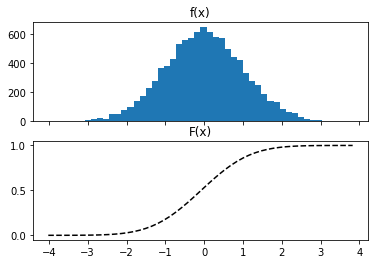
\includegraphics[width=8cm]{../figures/PdfCdf}
\caption{\label{fig:PdfCdf} Probability distribution function and cumulative distribution funtion of a normal distrubution.}
\end{center}
\end{figure}

We can then interpret the CDF as a new variable $s = F(t)$, meaning that $F$ becomes a transformation that maps $t$ to $s$, i.e. $F:t \to s$. Accordingly,  $\lim_{t \to -\infty}s(t) = 0$ and $\lim_{t \to \infty}s(t) = 1$ and $s$ can be intuitively interpreted as the fraction of the distribution of $t$ with values smaller than $t$ from the definition of the CDF. This implies that the probability distribution of $s$, $g(s)$, is constant in the interval $s\in [0,1]$ in which $s$ is defined and $s$ can be interpreted as the cumulative distribution of its own probability distribution:

\begin{equation}
s = G(s) = \int_{-\infty}^{s} g(s^\prime) ds^\prime
\end{equation}

In case of discrete probability functions such as the negative binomial function, the same argument still holds but the definition of the inverse quantile function is replaced by the generalized inverse: $F^{-1}(y) = \mathrm{\inf \left \{x : F(x)>y\right  \} }$ for $y \in [0,1]$, see e.g. \cite[p. 54]{casella2002statistical}. In order to obtain a uniform distribution for discrete PDFs that is comparable to the case of continuous distributions, the histogram holding the inverse quantiles or values of the CDF is filled using random numbers according to the intervals of the CDF. For example, if the sales of zero items accounts for 75\% of the observed sales distribution for this item, the value of the CDF function that is used to fill the histogram is randomly chosen in the interval $[0,0.75]$. Proceeding similarly for all other observed values, the resulting histogram of CDF values should again be uniform as in the case of a continuous PDF.

A histogram of the quantiles (or PIT values) of each prediction is therefore expected to be uniformly distributed in $[0,1]$ if the predicted probability distribution $f(x)$ is correctly calibrated.

This is illustrated in \fig \ref{fig:cdf_histos}, which shows the distribution of quantiles (or PIT values) for five different cases. If both the choice of the model and the model parameters are estimated correctly, we would expect the uniform distribution as shown in the last part of the figure. The first two plots of \fig \ref{fig:cdf_histos} indicate a bias in the variance estimation and the third and fourth plot indicate a bias in the mean
estimation.

\begin{figure}
\begin{center}
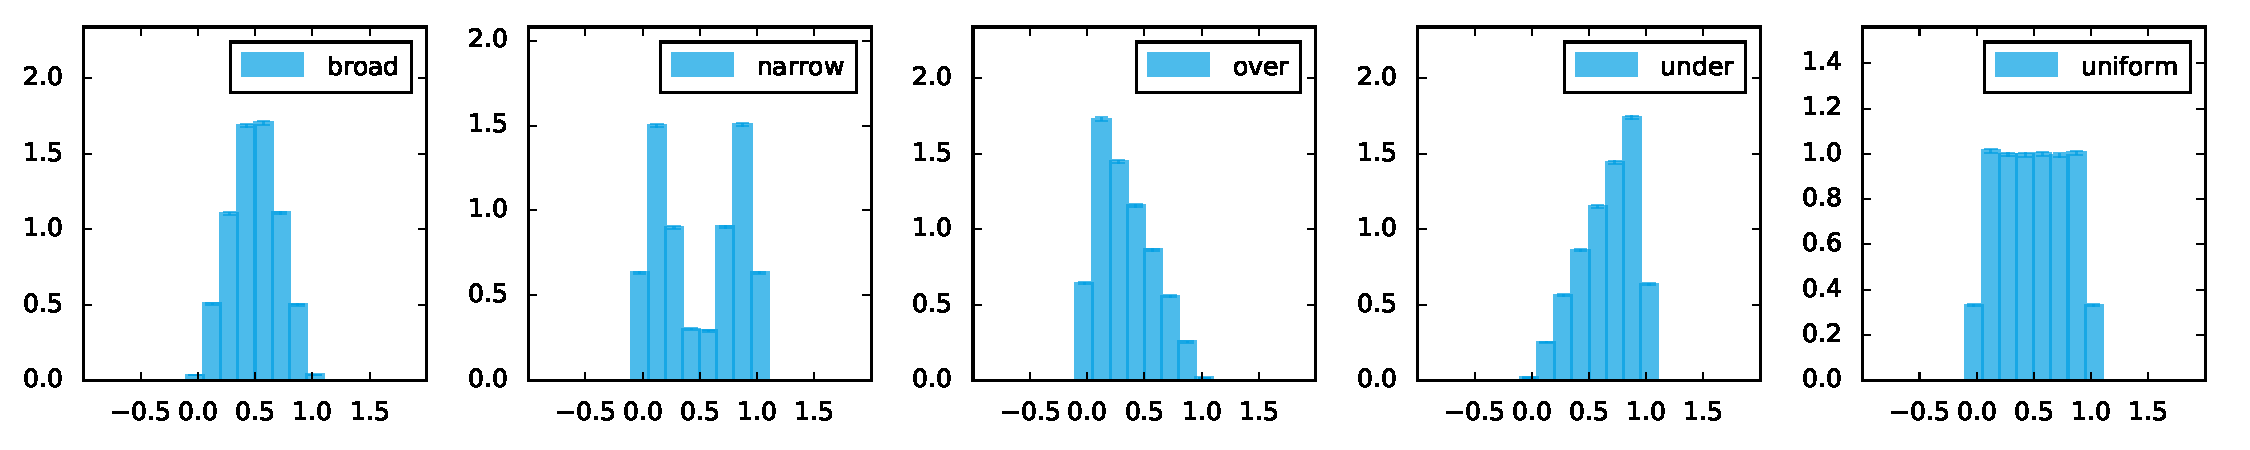
\includegraphics[width=8cm]{../figures/cdf_histos}
\caption{\label{fig:cdf_histos} ...}
\end{center}
\end{figure}

\subsubsection{Inverse Quantile Plot}
Evaluating the full probability function in the simplest case, where we have only one model that can be used to predict all observations, is straight-forward: We could fill a histogram of all observed values, such as sales records, and overlay this with the single model, such as a negative binomial with predicted parameters, that is used for all observations. Then, we could directly compare the model curve with the observations, using statistical tests such as the Kolmogorov-Smirnov test. In practical applications however, we have a large number of effective prediction models, since although we always use the same model parametrization, such as the negative binomial distribution, its parameters have to be determined at the required level of granularity. For example, for daily orders, we need to predict the parameters of the negative binomial distribution for each location, sales day, and product. Unlike the simple case discussed initially, where we had many observations to compare the prediction model to, we now have just one observation per prediction, meaning that we cannot use statistical tests directly. Instead we use the fact that a correctly calibrated, predicted PDF should return a uniform cumulative density distribution {\em regardless} of the shape of the predicted distribution.

We therefore proceed as follows: First, each individual predicted probability density distribution is transformed to its cumulative density distribution. In the example of the granularity from above, we would then have a CDF for each predicted PDF for each product, sales day, and sales location. The CDF values, also known as quantiles, of the corresponding truth values are then compared (in the sense of higher or lower) to expected quantile values and accordingly filled to a collection of profile plots, each of which representing one expected quantile value.

\fig \ref{fig:invquant_profiles} illustrates five different collections of inverse quantile profile plots (each collection comparing to 7 expected quantile values), each with only one bin for the sake of visualization, for separate sets of exemplary probability density estimation and observed data combinations. Each shown line represents the percentage of probability density estimation and observed data combinations for which the observed data point should be above and below the quantile of the predicted PDF indicated by that line (for example, the 0.50 line, corresponding to the median, indicates that 50 percent of all probability density estimation and observed data combinations in a given set of data should fall above the line, and 50 percent should fall below the line), respectively. The observation of the number of samples, indicated with shaded circles, that do in fact fall above and below a particular line, then allows the evaluation of the accuracy of probability density estimations. For a set of accurate PDF predictions, one expects a uniform shape, like illustrated by the final far-right column of shaded circles. Here, all shaded circles exactly fall on the line, indicating that both mean and variance estimations, as well as the choice of a negative binomial distribution as underlying PDF, were correct. Conversely, the leftmost two columns of shaded circles illustrate a case for which the variance estimation has a bias, and the center and center-right columns of shaded circles illustrate cases for which the mean estimation has a bias.

\begin{figure}
\begin{center}
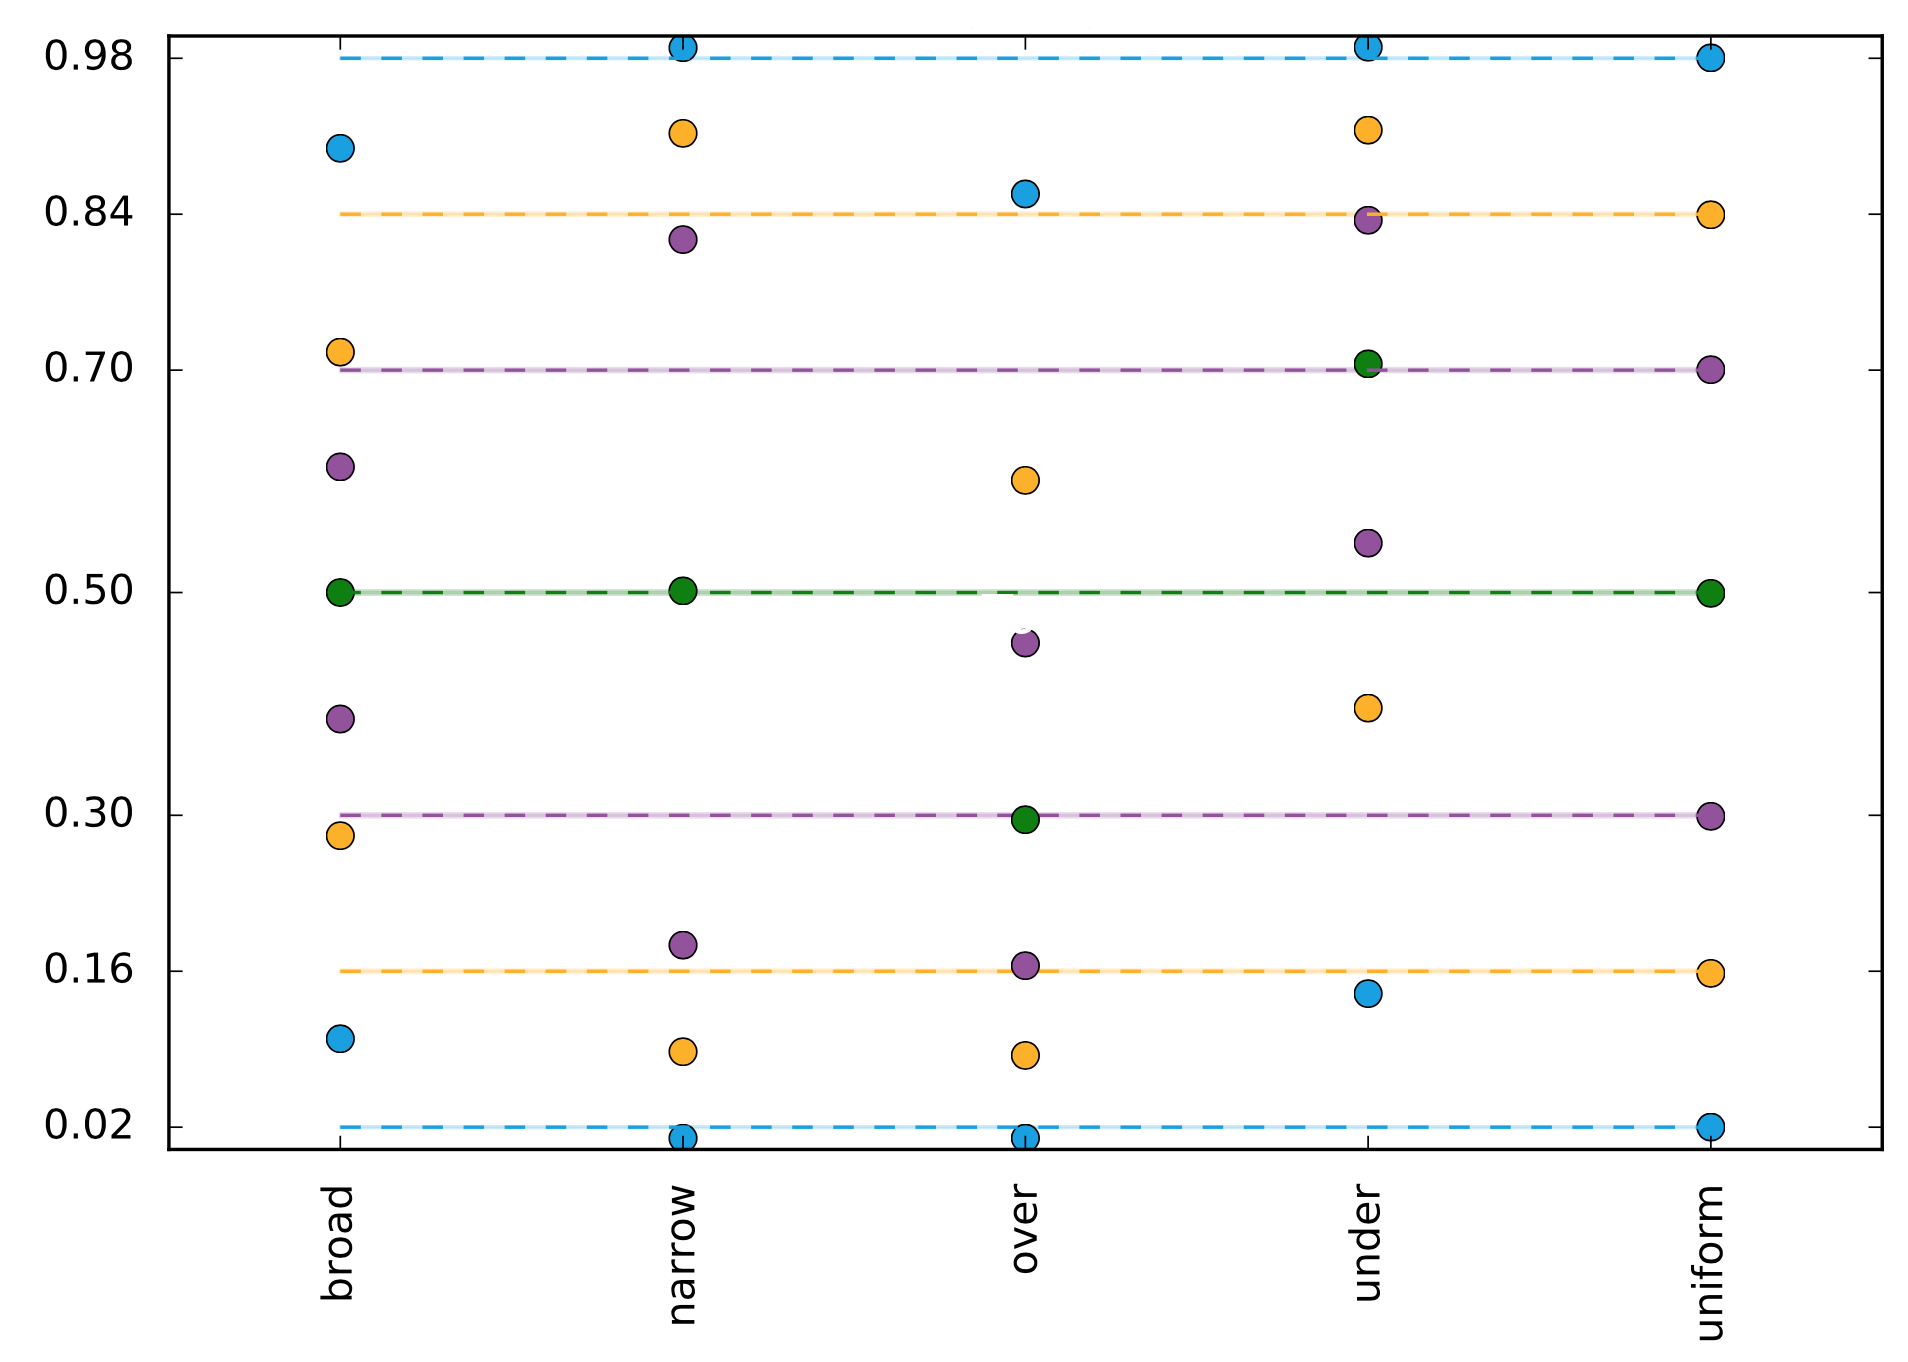
\includegraphics[width=8cm]{../figures/invquant_profiles}
\caption{\label{fig:invquant_profiles} ...}
\end{center}
\end{figure}

The two advantages of this method, as compared to the simpler method presented in section \ref{sec:cdf_histo}, are that an inverse quantile plot supports the qualitative evaluation of the predicted individual PDFs not only globally but (1) for different specified quantiles (potentially hinting to deviations in e.g. the tails of the distributions) and (2) in dependence of arbitrary variables of the data set (potentially hinting to deviations in e.g. specific categories of a feature). Two examples for this can be found in figures \ref{fig:invquant_mean} and \ref{fig:invquant_dayofweek} in the next section.

\subsection{Quantitative Evaluation of PDF Predictions}

The methods described so far allow a detailed qualitative evaluation of PDF predictions. However, in order to also quantify the quality of the PDF predictions, a measure of the deviation of the PDF predictions from the optimal outcome given the observed target data is needed. To achieve this, we compare the CDF histogram of the predicted PDFs with the uniform distribution and define a prediction accuracy interval between 0 and 1. Several different methods can be used to compute the deviance between two probability distributions. Good choices are the \textbf{1st Wasserstein distance} \cite{olkin1982}, the \textbf{Kullback-Leibler divergence} \cite{kullback1951}, and the \textbf{Jensen-Shannon divergence}  \cite{dagan1997}.

The 1st Wasserstein distance, also known as earth mover distance (EMD), represents a distance function defined between two probability distributions on a given metric space, and for our purposes here can defined by

\begin{equation}
\text{EMD}(P, Q) = 2 \cdot \frac{\sum_{k=1}^N |F_P(x_k) - F_Q(x_k)|}{N},
\end{equation}

where $F_P(X)$ and $F_Q(X)$ are the CDFs of the two PDFs $P(X)$ and $Q(X)$, respectively, and $x_k$ denotes the average value of $X$ in bin $k$, with $X$ being divided in $N$ bins.

The Kullback-Leibler divergence is a measure of how one probability distribution diverges from a second expected probability distribution. For PDFs $P(X)$ and $Q(X)$, again with $X$ being divided in $N$ bins $k$, the Kullback-Leibler divergence from Q to P is defined as

\begin{equation}
D_{\text{KL}}(P \parallel Q) = \sum _{k=1}^N P(x_k) \log \left({\frac{P(x_k)}{Q(x_k)}}\right),
\end{equation}

where $\log$ can be either base-2 or natural logarithm.

The Jensen-Shannon divergence (JSD) can be seen as a symmetrized and smoothed version of the Kullback-Leibler divergence:

\begin{equation}
D_{\text{JSD}}(P \parallel Q) = 0.5  \cdot (D_{\text{KL}}(P \parallel M) + D_{\text{KL}}(P \parallel M)),
\end{equation}

where $M = 0.5  \cdot (P + Q)$.

The EMD has the advantage over the mentioned divergences that it takes an underlying metric space into account, meaning that it depends on the distance of potential deviations.


\section{Example: Demand Forecasting}
\label{sec:example}

\textcolor{red}{... predict an individual demand volume for different product-location-date combinations ...}

\subsection{Mean and Variance Estimations}

\textcolor{red}{...}

\begin{figure}
\begin{center}
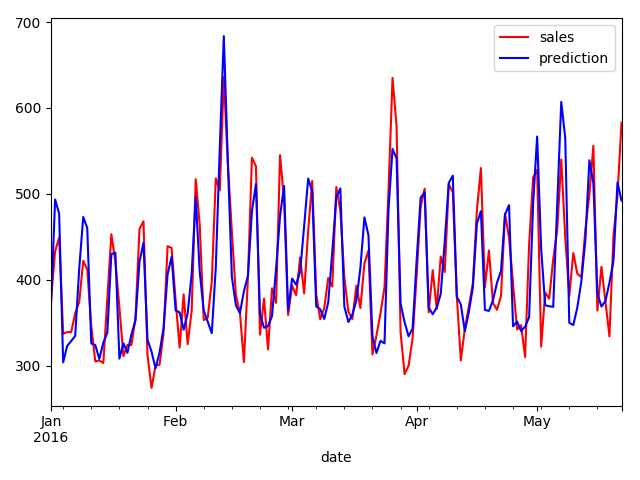
\includegraphics[width=8cm]{../figures/mean_prediction}
\caption{\label{fig:mean_prediction} time series of mean prediction and actuals for one item in all stores}
\end{center}
\end{figure}

\begin{figure}
\begin{center}
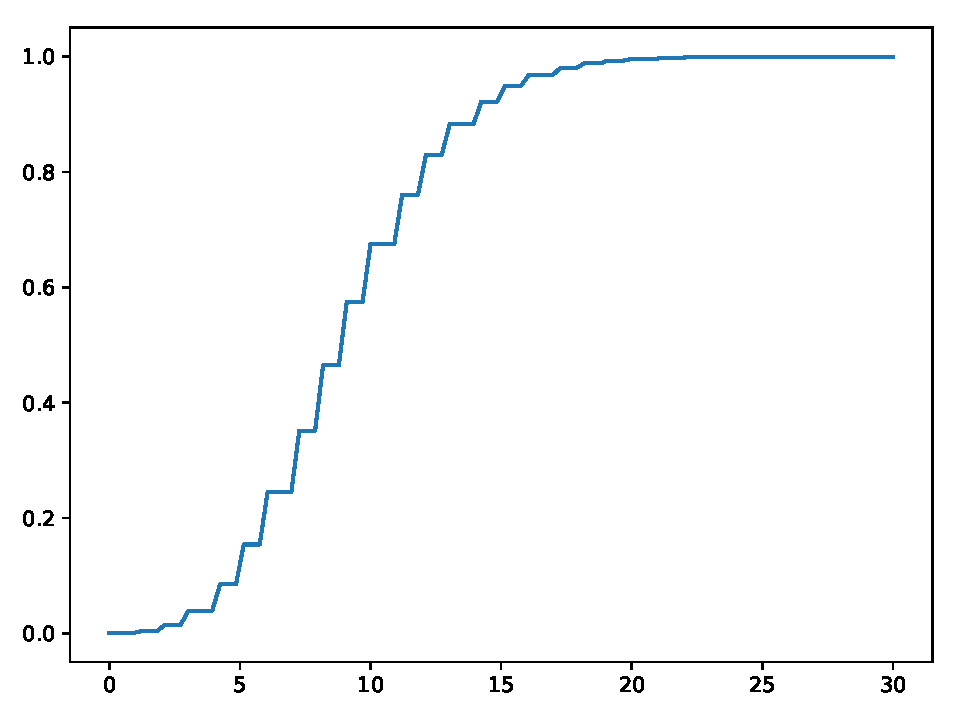
\includegraphics[width=8cm]{../figures/cdf}
\caption{\label{fig:cdf_example} CDF example}
\end{center}
\end{figure}

\subsection{Evaluation of PDF Predictions}

\textcolor{red}{...}

\begin{figure}
\begin{center}
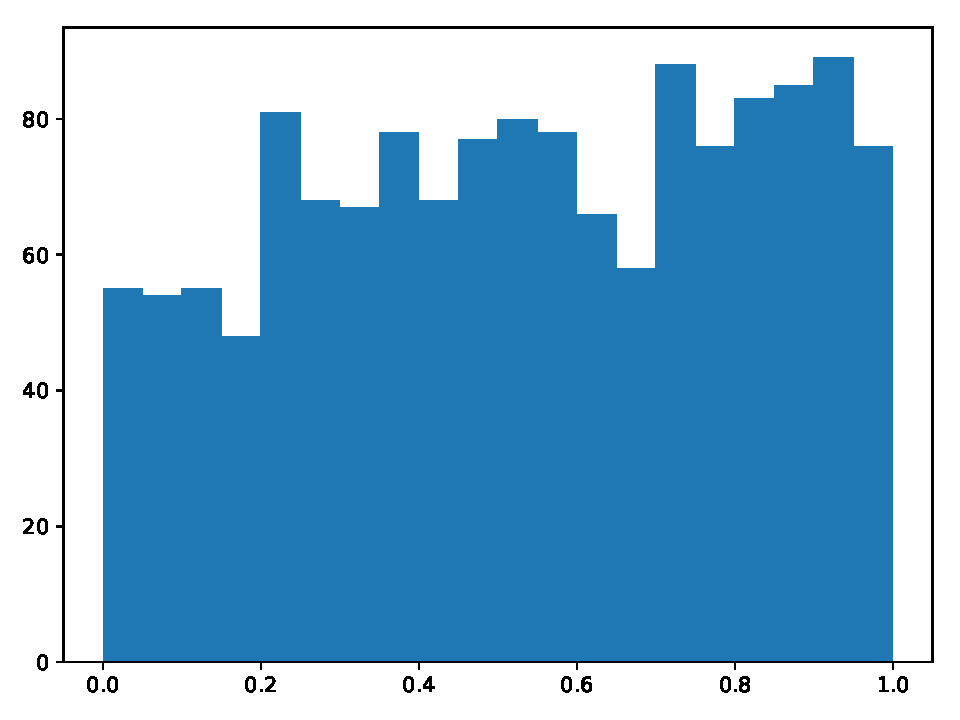
\includegraphics[width=8cm]{../figures/cdf_truth}
\caption{\label{fig:cdf_demand} CDF histogram}
\end{center}
\end{figure}

\begin{figure}
\begin{center}
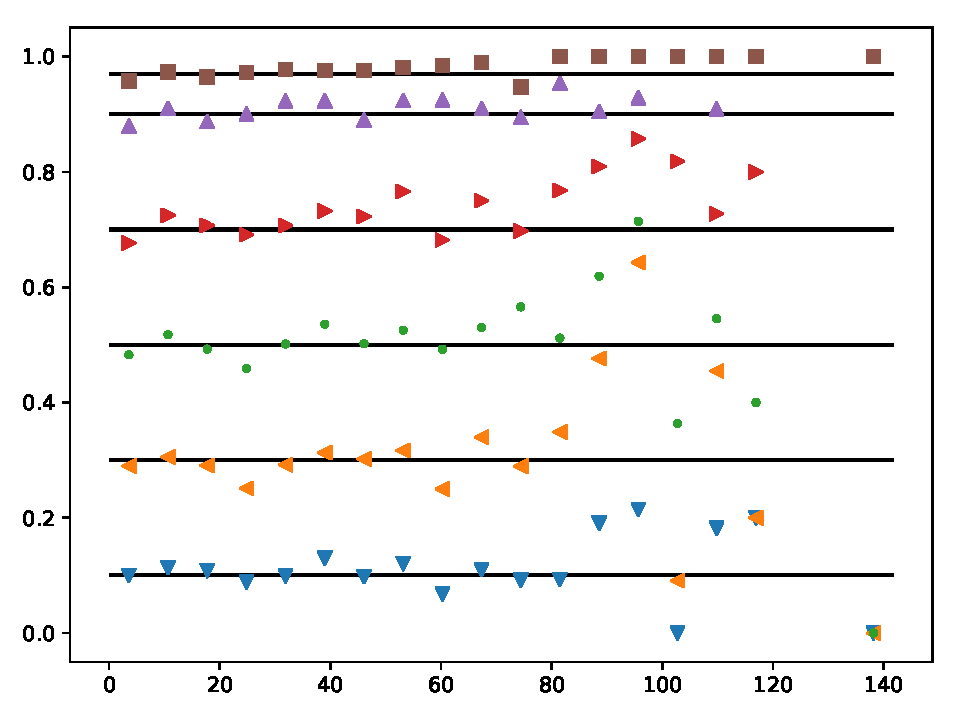
\includegraphics[width=8cm]{../figures/invquant_yhat_mean}
\caption{\label{fig:invquant_mean} invquant profile for mean prediction on X-axis}
\end{center}
\end{figure}

\begin{figure}
\begin{center}
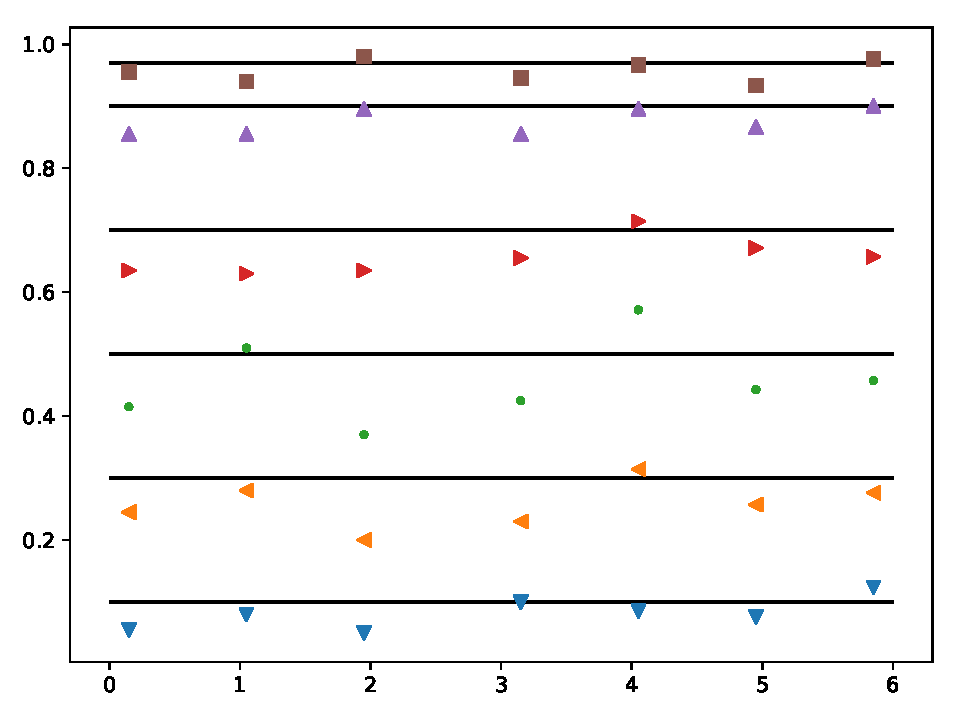
\includegraphics[width=8cm]{../figures/invquant_dayofweek}
\caption{\label{fig:invquant_dayofweek} invquant profile for day of week on X-axis}
\end{center}
\end{figure}

\textcolor{red}{... quantitative CDF accuracy ...}


\section{Conclusion}

We have shown how to use two subsequent machine learning models for mean and variance estimation together with a negative binomial model assumption to come up with individual PDF predictions. This setup is especially useful for retail demand forecasting, where the true demand follows a negative binomial distribution quite closely. Compared to a model-free approach like quantile regression, the distributional assumption therefore drastically reduces the uncertainty of the resulting predictions, which are, by using Cyclic Boosting as underlying machine learning algorithm, fully explainable on the individual level. 

Furthermore, we have presented new qualitative and quantitative methods for evaluating predictions in form of full PDFs. For qualitative evaluation, it is important to check the full PDF, especially its tails that are often crucial for subsequent decision making, as well as investigate aggregations of individual PDFs (to reduce the uncertainty of the evaluation) dependent on specific variables, and we have proposed a novel profile approach called inverse quantile plot for this. For quantitative evaluation, it is always desirable to have a single number to compare different models in terms of accuracy, and we have suggested to use the deviance between the CDF histogram of the predicted PDFs and the uniform distribution to compare PDF accuracies.


\bibliography{paper}
\bibliographystyle{ieeetr}

%%
%% Appendices
%%
\appendix

\section{Profile Histograms}

In many cases, scatter plots are used to study the behaviour of two distributions or sets of data points visually. However, even for moderate amount of data, this approach becomes quickly difficult. To illustrate this, a sample of $(x,y)$ data points was obtained in the following way: The distribution of $x$ values was obtained by generating 5,000 samples of Gaussian distributed random numbers $X \sim {\cal N}(0.0,2.0)$ and the $y$ values are obtained via $Y \sim X +  {\cal N}(2.0,1.5)$. \fig \ref{fig:scatter} shows the marginal distributions for $x$ and $y$ as well as a scatter plot of $x$ vs. $y$.

\begin{figure}
\begin{center}
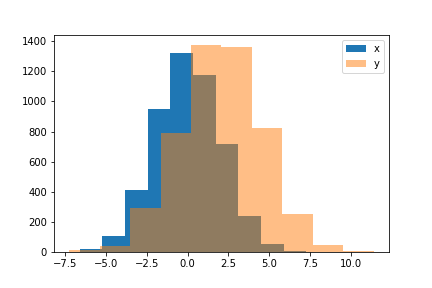
\includegraphics[scale=0.5]{../figures/marginal} 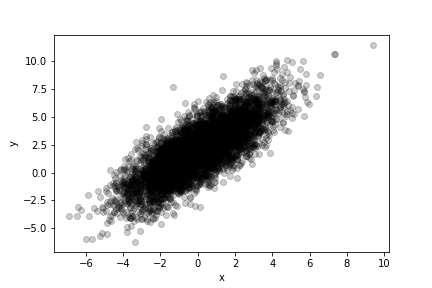
\includegraphics[scale=0.5]{../figures/scatter}
\caption{\label{fig:scatter} Marginal distribution and scatter plot of variables $X$ and $Y$.}
\end{center}
\end{figure}

Although the simple linear correlation between $X$ and $Y$ is apparent in the scatter plot, finer details are not visible and it is easy to imagine that a more complex relationship is difficult to discern. Profile histograms are specifically designed to address this shortcoming. Intuitively, profile histograms are a one-dimensional representation of the two-dimensional scatter plot and are obtained  in the following way: The variable on the $x$ axis is discretizised into a suitable range of bins. The exact choice of binning depends on the problem at hand. One can for example choose equidistant bins in the range of the $x$ axis or non-equidistant bins such that each bin contains the same number of observations. Then within each bin of the variable $X$, the a location and dispersion metric is calculated for the variable $Y$. This means that the bin-borders on the $X$ axis are used as constraints on the variable $Y$ and with these conditions applied, for example the sample mean of the selected $y$ values as well as the standard deviation are calculated. These location and dispersion metrics in each bin of $X$ are used to illustrate the behaviour of the variable $Y$ as the values of the variable $X$ change from bin to bin. The resulting profile histogram is shown in \fig \ref{fig:profile}. This one-dimensional representation allows to understand even a complex relationship between two variables visually. Note that due to few data points at the edges of the distributions the profile histogram is expected to show visual artifacts in the corresponding regions.

 \begin{figure}
\begin{center}
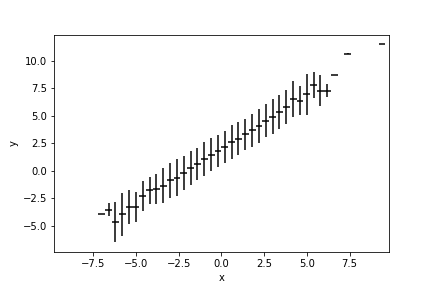
\includegraphics[scale=0.5]{../figures/profile}
\caption{\label{fig:profile} Profile histogram of variables $X$ and $Y$.}
\end{center}
\end{figure}


\end{document}
